\documentclass[a4paper,12pt,twocolumn]{article}
\usepackage[utf8]{inputenc}
\usepackage{graphicx}
\usepackage{hyperref}
\usepackage[margin=0.5in]{geometry}
\title{Logic Circuit of the Boolean Expression}
\author{Ginna Shreyani}
\date{August 2022}

\begin{document}

\maketitle

\section{Problem:}
Draw the Logic Circuit of the following Boolean Expression:\\
\begin{equation} (U'+V).(V'+W')\end{equation}
\maketitle
\section{Solution:}
\subsection{Theory:}
The logic circuit of the Boolean expression is designed by using logical gates. The logic gates we use for the given boolean expression are NOT, AND, NOR gates. With the help of truth table and the expression, the logic circuit is designed. \\
By simplifying the given equation we get the
following equation:\\
\begin{equation} Y=(U'.V')+(V.W')\end{equation}
Therefore, from equation (2), we can say that
there are two multiplications and an addition
operations in solving the given equation. As a
result, we use two AND gates for multiplication
operations and a single OR gate for addition.
\subsection{Truth Table:}
\begin{figure}[h]
\centering
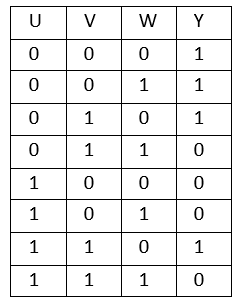
\includegraphics[width=0.4\columnwidth]{ttable}
\end{figure}
\begin{figure}[h]
\centering
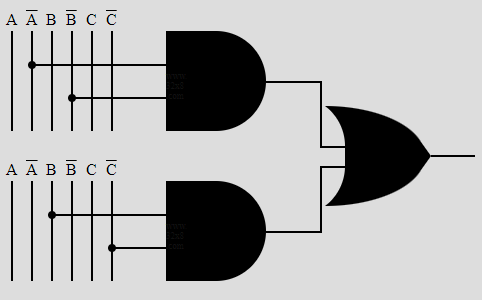
\includegraphics[width=0.5\columnwidth]{lc}
\label{Logic Circuit}
\caption{Logic circuit of the given boolean expression}
\end{figure}
\section{Hardware:}
\subsection{Components:}
\begin{figure}[h]
\centering
\includegraphics[width=0.5\columnwidth]{compo}
\end{figure}
\subsection{Connections:}
Arduino UNO has LED connected to Pin 13. Let pins 6,7,8 be the inputs. Connect the input pin to Vcc, if it must be set to '1'. Connect the input pin to GND of arduino board, if it must be set to '0'. The LED will glow if the output is '1'.
\section{Code:}
This is the source code\\
\href{https://github.com/ShreyaniReddy/IITH-FWC/blob/main/boolean.asm:}{Source code}

\end{document}
